\xchapter{Experimentos}{}

Nesta seção, mostrarei o resultado das medições de latência feitas no Raspberry. Os valores serão comparados entre diferentes versões do kernel, entre diferentes tipos de interrupções e com diferentes cargas da CPU.

\section{Configuração do kernel durante a compilação}

Para compilar os kernels usados estavam nas medições, foram usadas as seguintes configurações:

\begin{itemize}
    \item Suporte a \textit{timer} de alta resolução.
    \item Escalonador de frequência configurado como Performance para manter a CPU operando na frequência máxima para evitar flutuações devido a frequência de operação da CPU.
    \item Debugger do kernel desabilitado.
    \item Compactação de memória desabilitada.
    \item Alocação contígua de memória desabilitada.
\end{itemize}

Para o Preempt-RT, foi configurado também o modo de preempção como PREEMPT\_RT\_FULL. Os arquivos finais de configuração encontram-se no repositório do github \cite{Taian2019}.

\section{Configuração do teste}

As medidas foram agrupadas por tipo de kernel, tipo de interrupção e carga da CPU. Durante a construção deste trabalho, foram encontrados problemas na adaptação do INTSight com o Xenomai, detalhados no capítulo 5. Portanto, esta sessão abordará os resultados com o kernel Linux padrão e os resultados com o Preempt-RT. Essas configurações resultam em um total de 18 grupos de testes, detalhados abaixo. Cada grupo passou por uma bateria de medições. Em cada bateria, 50.000 medições foram realizadas com um intervalo de 20 ms entre elas.

O INTSight gera 2 arquivos no formato CSV para cada bateria de medição: um arquivo chamado \textit{name} e outro arquivo com o nome do tipo de contador usado. O arquivo \textit{name} contém o tipo de evento que acionou a coleta do contador do sistema e o arquivo com o nome do tipo de contador usado contém o valor do contador no momento em que a coleção foi acionada. Nos dois arquivos, cada medida ocupa uma linha do arquivo.

O repositório do INTSight fornece um script R que mescla esses arquivos em um único usando as seguintes informações: \textit{position} (posição do item na medição), \textit{run} (número da medição na bateria), \textit{name} (evento que acionou a medição), \textit{ktime\_mono\_fast} (valor do contador). Apesar desse script, o processamento de dados tem sido lento, pois gera \textit{dataframes} para os dados de entrada e os trata na memória até que tenha a saída final para salvar em disco. Como os \textit{dataframes} são muito grandes, mesmo em um computador com 12 GB de memória, ele começa a usar o disco para lidar com isso. Portanto, a lógica foi reescrita em um script Python que, ao tratar cada medição, salva o resultado diretamente em um arquivo CSV, ao invés de manipular \textit{dataframes}, reduzindo o tempo para tratar cada bateria de teste de 2 horas para 20 minutos. Para baterias de teste menores ou computadores com muita memória disponível, onde todos os dados cabem na memória, é aconselhável usar o script R fornecido.

Para consolidar os resultados das 18 baterias, um script Python foi criado usando o Apache Spark, um framework para lidar com big data \cite{Spark2009}. Embora nenhum tratamento de big data seja necessário para lidar com essa quantidade de dados, o Spark abstraiu parte da lógica, tornando o script mais simples. Esse script também filtra os dados úteis, pois o INTSight pode exibir valores zero quando ocorre um erro durante uma medição.

\section{Visão geral}

Para identificar as baterias de teste, um padrão de siglas foi adotado com o tipo de kernel, o tipo de mecanismo de interrupção e o indicador de carga da CPU. Por exemplo, a bateria de teste do kernel padrão Raspberry, com mecanismo Softirq e CPU com 0 threads de carga, tem a abreviação RS0. A bateria de teste do Preempt-RT, o mecanismo de Workqueue e a CPU com várias threads (\textit{many threads}), têm o acrônimo PWM. Várias threads nesse trabalho corresponde a 256 threads.

Na tabela \ref{table:rpi}, temos uma visão resumida do tempo de latência em nanossegundos de todos os testes realizados com o kernel padrão e na tabela \ref{table:prt}, temos uma visão resumida do tempo de latência dos testes executados com Preempt-RT.

\begin{table}[!p]
\centering
\begin{center}
\begin{tabular}{|c|r|r|r|r|r|r|r|r|r|}
\toprule
Percentil &    RS0 &     RS1 &    RSM &    RT0 &    RT1 &    RTM &    RW0 &     RW1 &      RWM \\
\midrule
    min &    833 &    365 &    781 &    625 &    938 &    573 &   7604 &    5730 &     5156 \\
    25\% &   1041 &    937 &    937 &   1145 &   1145 &   1146 &   8021 &    8073 &     8750 \\
    50\% &   1042 &    938 &    938 &   1146 &   1146 &   1146 &   8124 &    8177 &     8854 \\
    75\% &   1094 &    990 &    990 &   1198 &   1198 &   1250 &   8229 &    8802 &     8958 \\
    90\% &   1146 &   1094 &   1042 &   1302 &   1302 &   1406 &   8489 &    9011 &     9218 \\
    99\% &   6041 &   5677 &   5937 &   6250 &   6251 &   6198 &  16666 &   18021 &    18282 \\
  99.9\% &   6927 &   6406 &   7187 &   7188 &   8073 &  10677 &  30520 &   27917 &    25052 \\
    max &  15156 &  20365 &  19375 &  34998 &  25834 &  45260 &  84635 &  983798 &  4153458 \\
\bottomrule
\end{tabular}
\end{center}
\caption{Principais dados das medidas do kernel padrão}
\label{table:rpi}
\end{table}

\begin{table}[!p]
\centering
\begin{center}
\begin{tabular}{|c|r|r|r|r|r|r|r|r|r|}
\toprule
Percentil &    PS0 &    PS1 &    PSM &    PT0 &    PT1 &    PTM &    PW0 &     PW1 &    PWM \\
\midrule
  min &   1197 &   1146 &   1197 &   1614 &   1563 &   1614 &  11563 &  11562 &  11562 \\
  25\% &   1406 &   1406 &   1406 &   1823 &   1823 &   1823 &  12084 &  12031 &  12083 \\
  50\% &   1407 &   1407 &   1458 &   1875 &   1875 &   1875 &  12239 &  12135 &  12187 \\
  75\% &   1459 &   1458 &   1459 &   1927 &   1927 &   1875 &  12396 &  12291 &  12344 \\
  90\% &   1510 &   1510 &   1510 &   1980 &   1979 &   1927 &  12761 &  12605 &  12656 \\
  99\% &   1979 &   1823 &   1979 &   2447 &   3073 &   3125 &  21928 &  20313 &  19323 \\
99.9\% &   4896 &   4062 &   4844 &   5364 &   5781 &   5468 &  40677 &  46146 &  39843 \\
max &  18698 &  17656 &  17657 &  17343 &  16979 &  17865 &  80526 &  73854 &  86198 \\
\bottomrule
\end{tabular}
\end{center}
\caption{Principais dados das medidas do Preempt-RT}
\label{table:prt}
\end{table}

Podemos ver em \ref{table:rpi} que no kernel padrão, a carga na CPU não influencia significativamente a latência dos mecanismos Softirq e Tasklet. Esses mecanismos são tratados no modo kernel e espera-se que a carga da CPU dos aplicativos no modo usuário não afete realmente esse tratamento. No entanto, para o mecanismo de Workqueue, tratado por threads dedicados e sujeito ao escalonador do sistema operacional, o aumento na carga da CPU faz com que a latência do pior caso aumente significativamente.

Examinando o Preempt-RT através da tabela \ref{table:prt}, vemos que a carga da CPU também não influencia a latência dos mecanismos Softirq e de Tasklet, como no kernel padrão. No entanto, diferentemente do kernel padrão, no mecanismo Workqueue, a latência também não muda significativamente devido à carga da CPU. Isso torna o Preempt-RT muito mais previsível, independentemente da carga aplicada pelos processos do usuário.

\section{Análise comparativa}

Ao analisar sistemas de tempo real, o interesse é como o sistema poderá responder dentro de um limite de tempo na pior das hipóteses. Aqui vamos comparar a latência entre os kernels e como eles se comportam em seus extremos. Os gráficos nas seções a seguir mostram os valores de latência nos percentis de 90\% a 99,9\%. O valor máximo foi omitido da visualização, pois esses são picos muito distantes do valor do percentil 99,9\%, especialmente para o kernel padrão, dificultando a análise visual do comportamento do kernel. A análise do pior caso é feita separadamente.

\subsection{Softirq}

No gráfico \ref{grafico:softirq}, podemos ver como os dois kernels se comportam no tipo de interrupção Softirq. O Preempt-RT tem uma latência mais alta nos casos médios que permanecem até aproximadamente os percentis entre 94,5\% e 97,5\%. Nesse intervalo, a latência padrão do kernel começa a aumentar, enquanto o Preempt-RT permanece estável até o percentil 98,5\%.

\begin{figure}[!p]
    \centering
    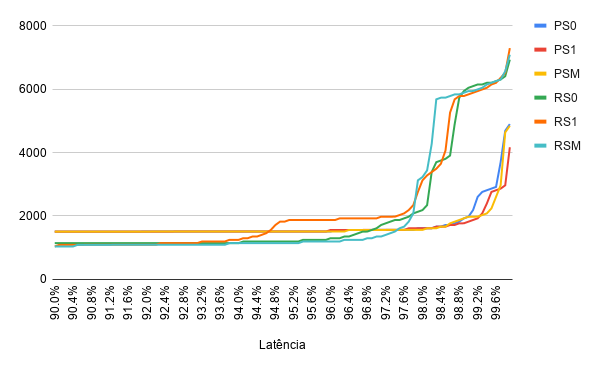
\includegraphics[width=\textwidth]{graficos/softirq.png}
    \caption{Latência com Softirq em nanossegundos}
    \label{grafico:softirq}
\end{figure}

\begin{table}[!p]
    \centering
    \begin{center}
        \begin{tabular}{|c|c|c|c|c|c|c|}
            \toprule
                Latência & PS0 &    PS1 &    PSM &    RS0 &     RS1 &    RSM \\
            \midrule
                máx & 18698 &  17656 &  17657 & 15156 &  20365 &  19375 \\
            \bottomrule
        \end{tabular}
    \end{center}
    \caption{Latência máxima para o Softirq}
    \label{table:max-softirq}
\end{table}

Para o pior caso de cada bateria de teste, temos a tabela \ref{table:max-softirq}. Nos casos com CPU ociosa, o Preempt-RT teve um tempo pior que o kernel padrão para o pior caso. Com a carga da CPU com 1 thread, o Preempt-RT teve uma leve redução no pior momento, enquanto o kernel padrão teve um aumento na latência. Com a CPU sobrecarregada, os dois kernels apresentaram valores próximos ao nível da CPU com carga de 1 thread.

Nos gráficos de dispersão para medições do Softirq no kernel padrão \ref{grafico:r-softirq} e Preempt-RT \ref{grafico:p-softirq}, podemos observar que existem muitos valores em uma faixa mais baixa e uma faixa menor com valores mais altos. O kernel padrão possui valores médios mais baixos para o intervalo inferior, mas possui um intervalo superior com valores mais altos. No Preempt-RT, a faixa superior está muito mais próxima da faixa inferior.

\begin{figure}[!p]
    \centering
    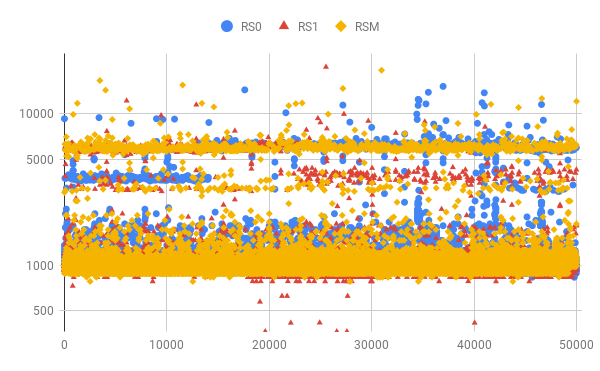
\includegraphics[width=\textwidth]{graficos/rs-scatter.png}
    \caption{Latência da bateria de testes com Softirq no kernel padrão}
    \label{grafico:r-softirq}
\end{figure}

\begin{figure}[!p]
    \centering
    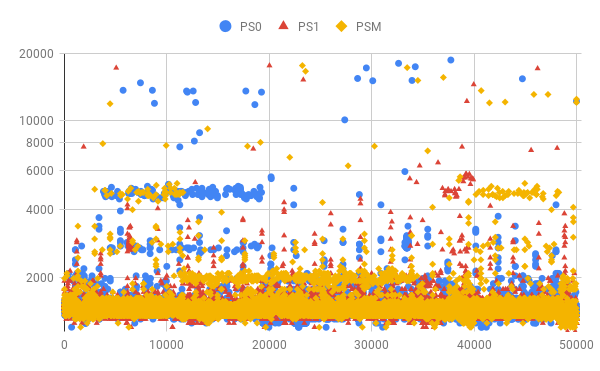
\includegraphics[width=\textwidth]{graficos/ps-scatter.png}
    \caption{Latência da bateria de testes com Softirq no Preempt-RT}
    \label{grafico:p-softirq}
\end{figure}

\subsection{Tasklet}

Para o tipo de interrupção Tasklet, os dois kernels se comportam de maneira semelhante ao Softirq, mas com uma latência um pouco maior, como podemos ver no gráfico \ref{grafico:tasklet}. O kernel padrão tem melhores tempos de resposta até aproximadamente 95\% quando possui carga na CPU ou em torno de 98\% quando a CPU está ociosa. Também na faixa de 98\% é quando o Preempt-RT começa a aumentar a latência.

\begin{figure}[!p]
    \centering
    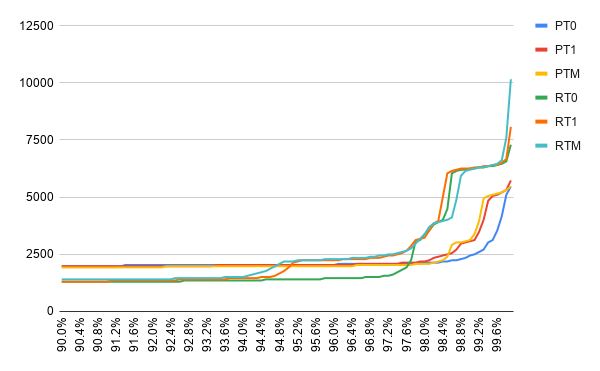
\includegraphics[width=\textwidth]{graficos/tasklet.png}
    \caption{Latência com Tasklet em nanossegundos}
    \label{grafico:tasklet}
\end{figure}

\begin{table}[!p]
    \centering
    \begin{center}
        \begin{tabular}{|r|r|r|r|r|r|}
            \toprule
                PT0 &    PT1 &    PTM &    RT0 &     RT1 &    RTM \\
            \midrule
                17343 &  16979 &  17865 & 34998 &  25834 &  45260  \\
            \bottomrule
        \end{tabular}
    \end{center}
    \caption{Latência máxima para o Tasklet}
    \label{table:max-tasklet}
\end{table}

Na tabela \ref{table:max-tasklet}, os valores de pior caso para os testes com o Tasklet. Podemos ver que o Preempt-RT quase não teve influência no nível de carga da CPU. No kernel padrão, há uma ligeira variação entre os valores, dependendo da carga imposta, mas ainda uma variação dentro de uma faixa não muito ampla.

Diferentemente do Softirq, a latência máxima do Tasklet no Preempt-RT é muito menor do que no kernel padrão. O Preempt-RT possui um tempo de resposta máximo que é quase metade do tempo do kernel padrão.

A dispersão do Tasklet é semelhante ao Softirq, como visto nos gráficos \ref{grafico:r-tasklet} e \ref{grafico:p-tasklet}. No kernel padrão, o número de valores que divergem do intervalo superior não parece ser maior que no Preempt-RT, mas os valores são mais distante da faixa comum.

\begin{figure}[!p]
    \centering
    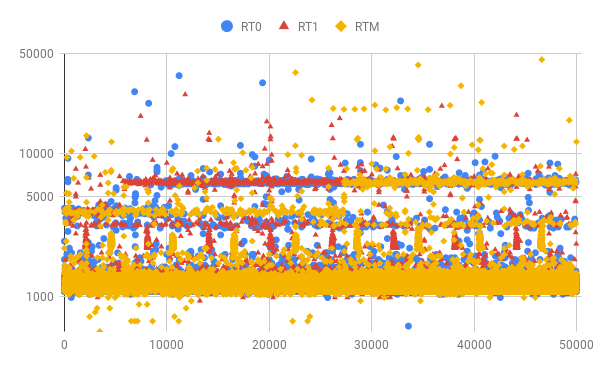
\includegraphics[width=\textwidth]{graficos/rt-scatter.png}
    \caption{Latência da bateria de testes com Tasklet no kernel padrão}
    \label{grafico:r-tasklet}
\end{figure}

\begin{figure}[!p]
    \centering
    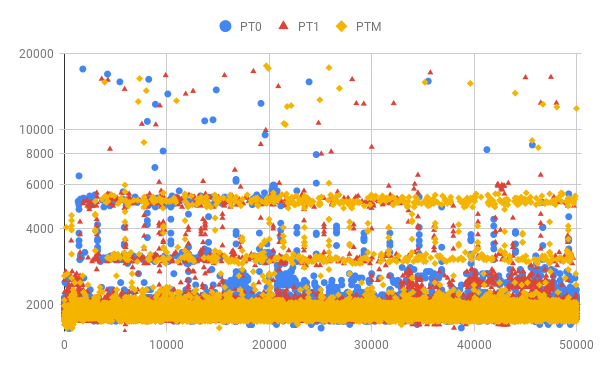
\includegraphics[width=\textwidth]{graficos/pt-scatter.png}
    \caption{Latência da bateria de testes com Tasklet no Preempt-RT}
    \label{grafico:p-tasklet}
\end{figure}

\subsection{Workqueue}

No tipo de interrupção Workqueue, as diferenças são sutis se o tempo máximo não for levado em consideração e a figura \ref{grafico:workqueue} mostra isso bem. Por outro lado, se formos analisar apenas o tempo máximo, a diferença entre os kernels é muito alta, como podemos ver na tabela \ref{table:max-workqueue}.

\begin{figure}[!p]
    \centering
    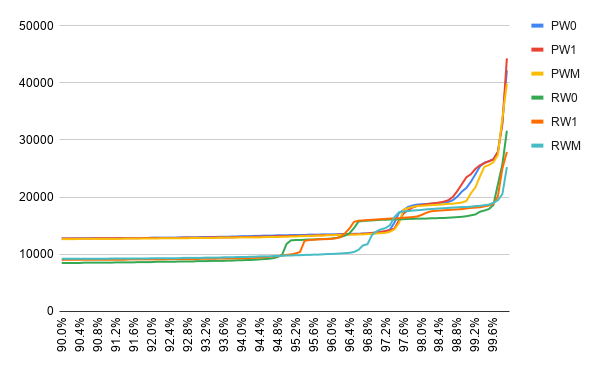
\includegraphics[width=\textwidth]{graficos/workqueue.png}
    \caption{Latência com Workqueue em nanossegundos}
    \label{grafico:workqueue}
\end{figure}

\begin{table}[!p]
    \centering
    \begin{center}
        \begin{tabular}{|r|r|r|r|r|r|}
            \toprule
                PW0 &    PS1 &    PWM &    RW0 &     RW1 &    RWM \\
            \midrule
                80526 &  73854 &  86198 & 84635 &  983798 &  4153458 \\
            \bottomrule
        \end{tabular}
    \end{center}
    \caption{Latência máxima para o Workqueue}
    \label{table:max-workqueue}
\end{table}

Ambos os kernels têm um tempo semelhante quando não há carga na CPU, mas com 1 thread de carga, o kernel padrão tem um tempo máximo mais de 10 vezes maior em comparação com a situação com a CPU ocioso. No Preempt-RT, há uma ligeira queda no tempo máximo.

Ao considerar uma CPU sobrecarregada, o tempo de Preempt-RT aumentou um pouco, mas permaneceu próximo aos valores da CPU sem carga. Já o kernel padrão, teve um tempo de resposta quase 50 vezes maior com sobrecarga da CPU em comparação com o cenário ocioso.

No gráfico \ref{grafico:r-workqueue}, podemos ver a dispersão das medições no Workqueue com as diferentes cargas. Podemos observar que, quando a CPU está sobrecarregada, a ocorrência de pontos fora da média ocorre mais de uma vez e com valores muito acima da média, tornando a latência não determinística.

\begin{figure}[!p]
    \centering
    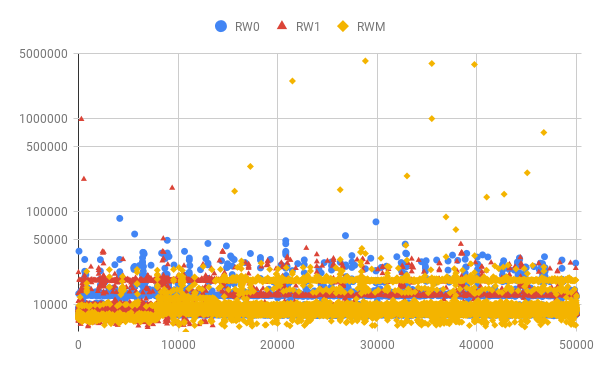
\includegraphics[width=\textwidth]{graficos/rw-scatter.png}
    \caption{Latência da bateria de testes com Workqueue no kernel padrão}
    \label{grafico:r-workqueue}
\end{figure}

Para o Preempt-RT, a dispersão é muito mais contida, como podemos ver no gráfico \ref{grafico:p-workqueue}. Os piores casos estão próximos um do outro e não tão longe da média. Não há valores que se afastem muito de um conjunto de valores que representa bem o grupo.

\begin{figure}[!p]
    \centering
    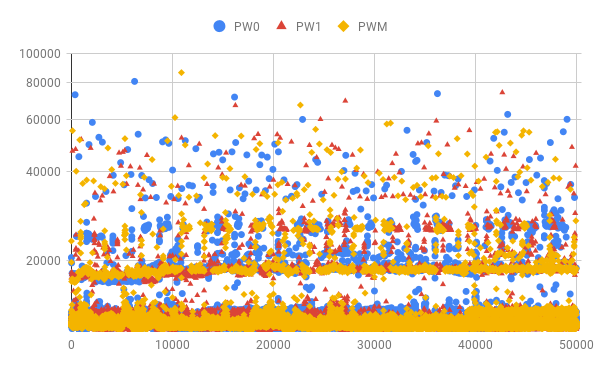
\includegraphics[width=\textwidth]{graficos/pw-scatter.png}
    \caption{Latência da bateria de testes com Workqueue no Preempt-RT}
    \label{grafico:p-workqueue}
\end{figure}

\section{Conclusões}

A implementação de um Softirq envolve a compilação de todo o kernel e não possui diferença significativa entre o kernel padrão e o Preempt-RT. Se for realmente necessário implementar a interrupção como Softirq, não há necessidade de usar o Preempt-RT, pois há um custo associado ao ter o kernel totalmente preemptivo.

Se optar por implementar a interrupção como Tasklet em um módulo do kernel, há diferenças na latência entre o kernel padrão e o Preempt-RT, sendo o Preempt-RT mais responsivo. No entanto, a variação na latência padrão do kernel com a carga da CPU não é tão grande. Se o pior caso medido for suficiente para atender às restrições de tempo do sistema, o kernel padrão poderá desempenhar o papel de sistema em tempo real sem onerar as demais tarefas.

Ao analisar o Workqueue, a diferença entre o kernel padrão e o Preempt-RT se torna evidente. Se a interrupção for implementada como fila de trabalho e for necessário um sistema que atenda às restrições de tempo, o Preempt-RT é a escolha a ser feita.
